\documentclass[sigplan,review,anonymous,10pt]{acmart}

% \acmSubmissionID{PAPER ID}
\renewcommand\footnotetextcopyrightpermission[1]{}
\settopmatter{printfolios=false,printacmref=false}

\usepackage{setspace}
\usepackage{enumerate}
\usepackage{algorithm2e}
\usepackage{algpseudocode}
\usepackage{graphics}
\usepackage{xparse} 
\usepackage{xspace}
\usepackage{multirow}
\usepackage{csvsimple}
\usepackage{balance}
\usepackage{minted}
\usepackage{xcolor}
\usepackage{nicefrac}
\usepackage{siunitx}
\usepackage{array,framed}
\usepackage{booktabs}
\usepackage{color}
\usepackage{soul}
\usepackage{float}
\usepackage{epsfig}
\usepackage{wrapfig}
\usepackage{graphics}
\usepackage{graphicx}
\usepackage{subcaption}
\usepackage{adjustbox}
\usepackage{csquotes}
\usepackage{cleveref}
\usepackage{dirtytalk}
\usepackage{textgreek}
\usepackage{oplotsymbl}
\usepackage{listings}
\usepackage{flushend}
\usepackage{float}

\setminted{
    fontsize=\small
  }


\def\eg{{\em e.g.}, }
\def\ie{{\em i.e.}, }
\def\etc{{\em etc.}\xspace}
\def\vs{{\em vs.}\xspace}

\def\gptmodel{{GPT-4o}\xspace}

\newcommand{\todo}[1]{\hl{\textbf{TODO:} #1}\xspace}
\newcommand{\sys}{{\scshape Kv{\textalpha}sir}\xspace}
\newcommand{\rf}[1]{\ref{#1}}
\newcommand{\sx}[1]{(\S\ref{#1})}
\newcommand{\cf}[1]{(\emph{Cf}.\S\ref{#1})}
\newcommand{\se}[1]{\S\ref{#1}}
\newcommand{\fg}[1]{Fig.~\ref{#1}}
\newcommand{\heading}[1]{\vspace{2pt}\noindent\textbf{\emph{#1}}:\enspace}
\newcommand{\ttt}[1]{\texttt{#1}\xspace}
\newcommand{\xxx}{\colorbox{red!30}{xxx}\xspace}
\newcommand{\promptbox}[1]{%
  \vspace{0.5em}%
  \hspace*{-0.0135\columnwidth}%
  \fbox{%
    \parbox[t]{0.95\columnwidth}{\tt #1}%
  }%
  \vspace{0.5em} % adjust this value as desired
}

\crefformat{section}{\S#2#1#3}
\crefmultiformat{section}{\S#2#1#3}{--\S#2#1#3}{, \S#2#1#3}{ and \S#2#1#3}

\setlength{\intextsep}{0pt} % vertical space above/below
\setlength{\columnsep}{5pt} % horizontal space between text and figure

\begin{document}


\title{\sys: Controllable Program Regeneration}
\author{Evangelos Lamprou}


% Use cases for something like this include:
% - program repair
% - turning insecure code into secure code by removing side-effects
% - transforming a program in language A to language B
% - turning a program into a more idiomatic version of the same language
% - having a program use a different API
% - have a program be more amendable to parallelization
% - have a program be more amendable to further analysis or transformation

\begin{abstract}
  Software evolution tasks---like security hardening, porting critical components to safer 
  languages, or refactoring opaque legacy code---are brittle and time-consuming.
  Large language models (LLMs) have shown promise in automating such tasks,
  but their outputs are shaped by surface cues, lack
  semantic guarantees, and their usage often boil down to brittle prompting strategies.
This paper presents \sys, a system for controllable program regeneration that
  combines declarative property constraints with LLM-guided synthesis. Unlike
  prior approaches, \sys treats the input program as an untrusted artifact and
  explicitly projects it into a minimal set of verifiable properties, such as
  input/output behavior, execution traces, and API signatures. These properties
  serve as constraints during synthesis and are checked post hoc to ensure
  correctness.
\sys is evaluated on a diverse set of program transformation tasks
including security hardening, language translation, idiomatic rewriting, de-obfuscation,
and modular refactoring showing strong results, even on tasks where state-of-the-art LLMs fail.
\end{abstract}

% Since this is a position paper (and not a tool paper), I would spend most of the paper selling the Idea, and less on the system and language. I think the examples does this well (but the language still feels a little too magical).
% The second section should probably focus on problem (program to program transformations) and the gab (related work), explaining why current approaches fall short.
% The third section should introduce our idea for a better solution, with examples. I think the core of the idea is building a knowledge base of the programs which we want to transform between, and then use (out of many) an LLM as an imperfect bidirectional analysis.
% I think the idea of bidirectional analysis is somewhat new, and handeling imperfect information in a logical system is not easy. I think we need to address why we think this is possible.
% The fourth section could contain a plan for future work: implementation and evaluation.
% The fifth section is a discussion and conclusion.

\maketitle

\section{Introduction}
% \begin{figure}[t]
%   % https://docs.google.com/drawings/d/1LAmdVYjfAID24eSM-hl5PRhVg9fRMJMWYETsvvcyAuU/edit?usp=sharing
%   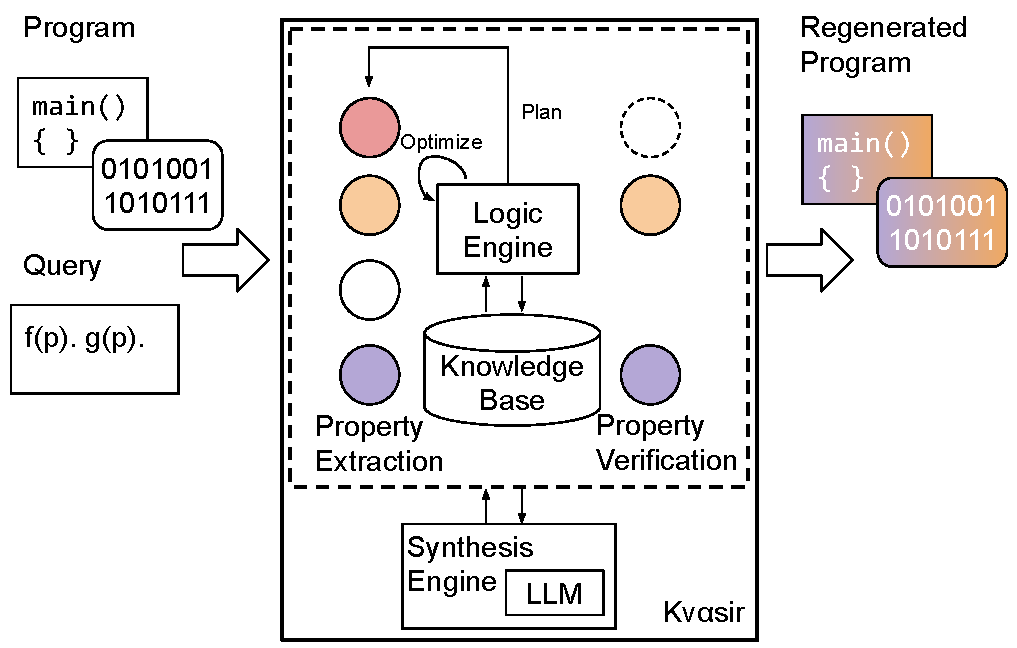
\includegraphics[width=.9\columnwidth]{figs/kvasir_overview.pdf}
%   \caption{\textbf{\sys overview}
% Given a transformation query, and a source program, \sys extracts a minimal set
%   of properties,
%   guided by a logic engine and knowledge base.
%   It then synthesizes a new program $P'$ that satisfies the query, verifying
%   that wanted properties are present and unwanted properties are absent in $P'$.
% }
%   \label{fig:overview}
% \end{figure}

\begin{figure}[t]
  % https://docs.google.com/drawings/d/1ozMu2B0RUhyLWC_rM6GLBrioov80-M06CBqYRAhCk18/edit
  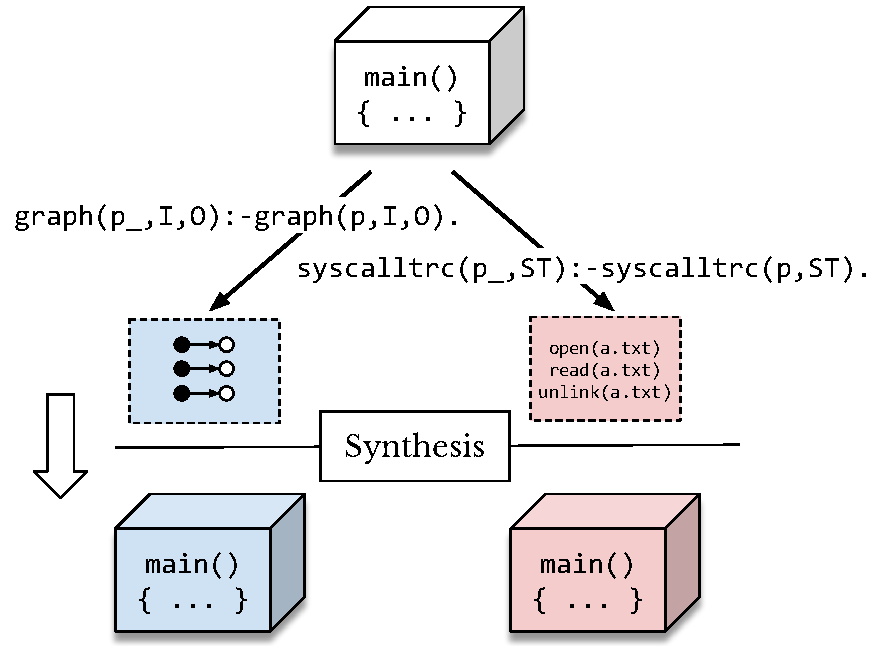
\includegraphics[width=.9\columnwidth]{figs/kvasir_projection.pdf}
  \caption{\textbf{Property projection and verifiable regeneration in \sys.}
  Instead of transforming source code directly, \sys projects the original
  program into a minimal set of verifiable properties---such as input/output
  examples, system call traces, \etc.
  These properties serve as declarative
  constraints for synthesis.
  The regenerated implementation is then checked to
  ensure it satisfies the specified properties, providing a verifiable
  foundation for trust unlike purely prompt-based LLM workflows.}
  \label{fig:projection}
\end{figure}


% insights: modular programs, advances in LLMs, need for a strictly declarative interface

% Mention that:
% 1. They have shown great promise in program synthesis + 
% 2. They can not do negative reasoning well - 
% 3. Their output are often closely aligned to their inputs. They are gullible (susceptible to adversarial inputs). -
% 4. Difficult to verify correctness of outputs against certain properties. The
%    user cannot easily set requirements or say output should be within a range of
%    acceptance


Modern software systems evolve constantly.
Developers refactor legacy code~\cite{Fowler99,Mens04,facebook2010redesigns,dropbox2014syncengine},
adapt libraries to changing APIs~\cite{dig2005role,kula2017empiricalstudyimpactrefactoring},
translate components across languages~\cite{manzoor_cli_python,gaultier_rewrite_cpp},
% and patch security vulnerabilities~\cite{ikegami2022userefactoringsecurityvulnerability,schneier2013security_vulnerabilities}.
These transformations, are often brittle, time-consuming, and require significant expertise.

Recent advances in natural-language processing, particularly large language
models (LLMs) have opened new possibilities for automating program
transformation and synthesis tasks,
making them attractive tools for software
evolution, albeit with caveats.
This flexibility has positioned them as attractive tools for software evolution
compared to traditional program synthesis techniques, which often struggle
to scale to real-world settings or across languages and require significant developer involvement~\cite{reynolds2019syguscomp,leino2016dafny,wu2023programming,dynamoth2016,cambronero2019active}.
LLMs can translate code across languages~\cite{ou2025enhancingllmbasedcodetranslation},
refactor complex modules~\cite{ziftci2025migrating},
and even generate entire components from scratch~\cite{huynh2025largelanguagemodelscode}.
However, surface-level patterns in the input shape their outputs~\cite{yang2025evaluatinggeneralizationcapabilitieslarge},
they struggle with negative constraints~\cite{hwang2024thinkpinkelephant,jiang2024llmsdreamelephantswhen},
often overfit to spurious input cues~\cite{xu2023llmfoolitselfpromptbased, wu2023deceptpromptexploitingllmdrivencode},
and lack mechanisms for enforcing precise behavioral properties on the generated code~\cite{roh2025breakthechainreasoningfailuresllms}.
As a result, developers must prompt and steer them through brittle heuristics or manual trial-and-error, leading to workflows that are difficult to audit, integrate, or systematically reason about.
Bridging this gap calls for an that allows developers to specify explicit semantic constraints and transformation goals, and to reason about their satisfaction in a principled way.

This paper explores the feasibility of combining declarative property
constraints with LLM-based synthesis to support \emph{property-guided program regeneration}.
The key idea is to treat the original program as an untrusted reference from
which to extract minimal, verifiable properties (\eg I/O behavior,
function signatures, program traces), and to synthesize a new implementation that satisfies those
constraints without overfitting to potentially spurious details of the original source code.
The engine for this experimentation is the \sys prototype.
\sys allows users
to express transformation goals declaratively, as logical constraints over
program properties.
At a high level, given a source program and a query, \sys uses the provided
logical constraints and its internal knowledge base to extract a set of
feasible and relevant program properties.
It then prompts an LLM to synthesize
candidate programs, which are subsequently verified against the desired properties.
This approach treats program transformation as projecting the original program over key properties.
Intuitively, regeneration then leverages LLM's high-dimensional internal representation~\cite{jin2024emergent,tao2024llms,huh2024platonicrepresentationhypothesis}, 
which lifts the projection back to a concrete implementation~(\cref{fig:projection}).
Unlike prompt-based approaches that require
extensive curation of examples~\cite{dilhara2024unprecedented, khattab2023dspy, cummins2024donttransformcodecode},
\sys treats the input program as an
untrusted artifact and explicitly projects only minimal, verifiable properties
into the regeneration process.

Three key insights shape the design of \sys.
First, modern software is highly decomposable~\cite{vfunction2024modular, isoline2018decomposition, schechter2011visualizing, breakapp:ndss:2018}, making it feasible to reason about transformations at the granularity of individual modules, libraries, or functions.
Second, the program \emph{regeneration} setting provides a unique advantage: the original program serves as a concrete ground-truth, enabling semantic comparisons and verification of the transformed output, something impossible in traditional synthesis tasks.
Third, the underlying synthesis technology---particularly LLMs---is evolving rapidly; a declarative interface harnesses this progress without disrupting the framework's end user.

% Guided by these insights, \sys casts transformation as a constrained synthesis problem.
% At its core is a property-driven pipeline: users express goals as logical constraints over semantic properties, such as input/output behavior, side-effect freedom, target language, or structural modularity.
% \sys extracts a set of relevant properties, derived from its logic engine and a domain-aware knowledge base, and synthesizes a new program that satisfies the specified constraints.
% If no such program exists, \sys returns a failure explanation from the unsatisfiable core.

\heading{Deployment scenarios and limitations}
\sys supports a range of deployment scenarios.
It is particularly well-suited for use during maintenance and auditing phases, where developers seek to refactor or replace components, especially when the original code is difficult to understand, modify, or is unavailable and the component exists only as a binary.
It can also assist during development, for instance when integrating
third-party modules that must be adapted to local conventions or hardened
against security vulnerabilities.
For example, a developer can regenerate a C library as idiomatic
JavaScript while preserving I/O equivalence, or decompose a monolithic function
into modular components suitable for sandboxing.
However, \sys is not designed for whole-program synthesis or large-scale migrations.
Its strength lies in scoped regeneration tasks, typically at the granularity of a function, method, or small module---where transformation goals can be explicitly stated and verified in isolation.
To this end, \sys can function not only as a standalone tool but also as a
library, where other components can invoke it as a programmable,
constraint-guided regeneration module.

% Leverages insights: (1) modern applications highly modular (2) the problem of LLM-assisted program transformations needs to be transformed in a way that a ground truth is readily available: the original program
% (3) towards the generality and longevity of this solution the interface needs to be purely declarative, to allow independent progress of the underlying components to give automatic benefits

% \heading{Contributions}
% The paper's contributions are:
% \begin{itemize}
%  \item A property-aware transformation framework, combining logic-based reasoning, and LLM-assisted program synthesis~(\cref{sec:design});
%  \item A declarative interface and accompanying DSL for program transformation, allowing users to express semantic goals as logical queries over properties of the regenerated program~(\cref{sec:dsl});
%  \item A verification architecture that checks synthesized programs against the specified properties, providing feedback for refinement~(\cref{sec:verification});
%  \item An empirical evaluation demonstrating \sys's feasibility across transformation scenarios~(\cref{sec:evaluation}).
% \end{itemize}

\section{Example}
\label{sec:example}

\begin{figure}[t]
\centering
  % https://docs.google.com/drawings/d/1zMcTurJ8twCG4BrkSUAJersbNSl5UQkogHqqg88vG9M/edit
  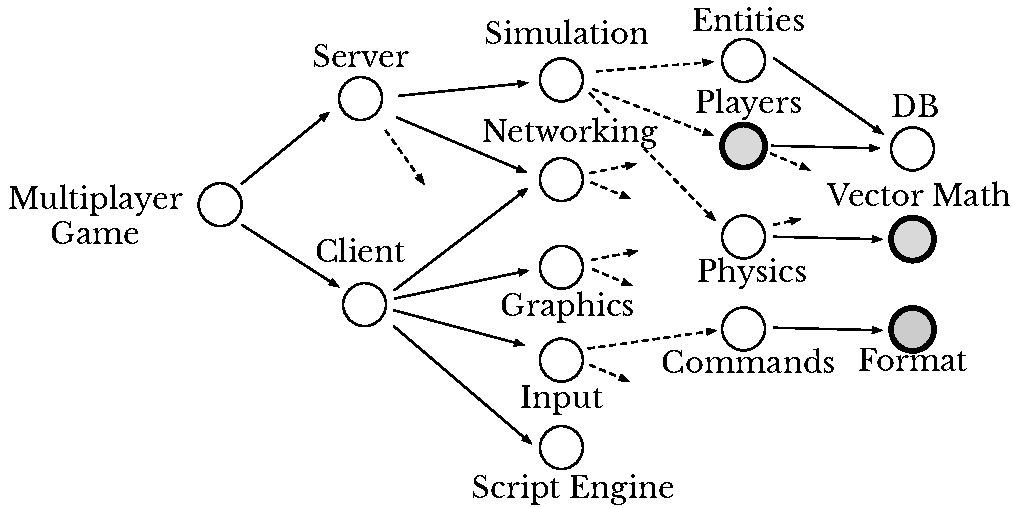
\includegraphics[width=.9\columnwidth]{figs/kvasir_application.pdf}
  \caption{\textbf{Applying \sys to a complex game application.}
  The high level of modularity present in modern applications allows \sys to be applied effectively across a codebase.
  Edges signify logical dependencies between components 
  and shaded vertices signify parts of the codebase \sys is applied as part of the example~(\cref{sec:example}).
  Dotted edges signify ommited layers of dependencies.
  }
  \label{fig:ex-large-app}
\end{figure}

This examples illustrates the capabilities of \sys by applying it to a representative game
application.
This example is selected to highlight the
diversity of transformation goals that arise even within a single codebase:
security hardening, cross-language migration, modernization of unsafe idioms,
and structural refactoring.

\heading{A legacy input handling function}
Zooming into the \ttt{cmd.c} file of the game codebase, 
which handles parsing and executing user commands provided by an in-game console.
This functionality is used by developers to test and debug the game, but also during regular gameplay
by game administrators or players where they can customize the game by spawning objects, changing game settings, \etc.
Such code is often notoriously difficult to write,
and there have been many instances of buffer overflow vulnerabilities being introduced because of it~\cite{CVE-2006-3400, CVE-2006-3401, CVE-2007-5248, CVE-2019-1010043}.
\begin{listing}
\begin{minted}[]{js}
#define MAX_C 1024
char *Cmd_Args(int argc, char **argv) {
 static char args[MAX_C];
 for (int i = 1; i < argc; i++) {
  strcat(args, argv[i]);
  if (i < argc - 1) strcat(args, " "); }
 return args; }
\end{minted}
\caption{A string formatting function that concatenates command-line arguments into a single string.}
\end{listing}

\begin{wrapfigure}[4]{r}{.64\columnwidth}
\begin{minted}{prolog}
fsignt(p_, S) :- fsignt(p, S).
graph(p_, I, O) :- graph(p, I, O),
                   crash(p, I).
:- crash(p_, I), graph(p_, I, _).
\end{minted}
\end{wrapfigure}
To the right is a program written in the \sys DSL to express this intent.
This query requires the regenerated program \texttt{P\_} to exhibit the same
I/O behavior on representative inputs that would cause a buffer overflow in the original program $P$.
but not on the regenerated program $P^\prime$.
\sys first arrives the set of properties to extract from the
original program, given the query:
$\{\ttt{input(P, I)}, \ttt{graph(P, I, O)}, \ttt{signature(P, S)}\}$, where
\texttt{input(P, I)} means that \sys will use extract a set of inputs from the original program
by prompting an LLM with the program's source code and asking it to generate a set of inputs that
would cause a buffer overflow in the original program;
\texttt{graph(P, I, O)} extracts the client-observable I/O behavior of the program
by executing the original program on the generated inputs and recording the outputs;
and \texttt{signature(P, S)} extracts each function's signature using a language-aware parser.

After 30.4 seconds and one attempt, \sys synthesizes the following program:
\begin{minted}[]{js}
#define MAX_C 1024
char *Args(int argc, char **argv) {
static char args[MAX_C];
int i; size_t remaining = MAX_C - 1;
args[0] = 0;
for (i = 1; i < argc; i++) {
  strncat(args, argv[i], remaining);
  remaining = MAX_C - strlen(args) - 1;
  if (i != argc - 1 && remaining > 0) {
    strncat(args, " ", remaining);
    remaining = MAX_C - strlen(args) - 1;
  } }
  return args; }
\end{minted}

Building on the same source as the previous example, \sys can perform
cross-language translation.
In this scenario, the developer aims to lift input
handling logic into a sandboxed JavaScript runtime to allow controlled
developer hooks and runtime customization, while reducing the attack surface of
the C runtime.
By moving this function into the scripting environment, it
becomes easier to enforce memory safety and auditability constraints.

\begin{wrapfigure}[5]{r}{.46\columnwidth}
\begin{minted}{prolog}
language(p_, javascript).
graph(p_, Ijs, Ojs) :-
     graph(p, Ic, Oc),
llm_translate(Ic, Ijs),
llm_translate(Oc, Ijs).
\end{minted}
\end{wrapfigure}
The query specifies that the regenerated program \texttt{P\_} must be
implemented in JavaScript and must preserve observable behavior over a
representative set of inputs and outputs.
To bridge differences in
representation between C and JavaScript, the query uses \texttt{llm\_translate}
to convert each input and output into equivalent forms suitable for the target language.
\sys first determines the minimal set of properties to extract from the
original function: $\{\texttt{graph(P, I, O)}\}$.
It then invokes \texttt{llm\_translate} to produce
corresponding JavaScript representations of each example input and output, such
that the translated function will reproduce identical string formatting
behavior.
After 29.4 seconds, having generated 20 translated input-output pairs, \sys synthesizes the following JavaScript function:

\begin{minted}{javascript}
function cmdArgs(argv) {
    return argv.slice(1).join(" ");
}
\end{minted}
Notice that the regenerated program has a slightly different signature than the original, 
since JavaScript arrays include built-in information about their length,
which makes the \ttt{argc} argument obsolete.
The synthesis backend had the freedom to make this change since the query did not specify a signature property.

\heading{An unidiomatic C function in a physics library}
The fast inverse square root routine, originally developed for the Quake III
engine~\cite{fast_inv_sqrt}, is included in the game's physics and vector math
library as an optimization for computing normalized vectors.
The implementation
exploits type punning to manipulate IEEE floats at the bit level—a technique
that relies on undefined behavior and reduces portability:
\begin{listing}
\begin{minted}{c}
float Q_rsqrt(float number) {
 long i; float x2, y;
 const float threehalfs = 1.5F;
 x2 = number * 0.5F; y  = number;
 i  = * ( long * ) &y; // evil bit level hack
 i  = 0x5f3759df - ( i >> 1 );
 y  = * ( float * ) &i;
 y  = y * ( threehalfs - ( x2 * y * y ) );
 return y; }
\end{minted}
\caption{An unidiomatic C implementation of the fast inverse square root function popularized by the game Quake III~\cite{fast_inv_sqrt}.}
\end{listing}
The query to the right uses lines of code as a coarse metric of
idiomaticity. \sys regenerates the program, minimizing this metric while
preserving observable behavior over a representative set of inputs which will be generated by an LLM instance.
\begin{wrapfigure}[2]{r}{.7\columnwidth}
  \begin{minted}{prolog}
graph(p_, I, O) :- graph(p, I, O).
#min N: len(p_, N).
  \end{minted}
\end{wrapfigure}
\sys extracts the set of properties \texttt{signature(F)} and \texttt{graph(F)}
from the original function, where \texttt{signature(F)} is the function's
signature (including its name, return type, and arguments) and
\texttt{graph(F)} captures the I/O behavior on a generated set of
floating-point inputs.
In this case, where the goal is to optimize an aspect of the program, \sys
re-prompts the model to regenerate the program until it can make no further
improvements or observes a negligible difference after two consecutive
iterations.

After 15.2 seconds and two iterations, \sys synthesizes the following idiomatic and portable version:
\begin{minted}{c}
#include <math.h>
float Q_rsqrt(float number) {
    return 1.0f / sqrtf(number); }
\end{minted}
The regenerated implementation is easier to verify, portable across compilers, and avoids undefined behavior.

\heading{A monolithic gameplay function}
Consider a JavaScript function in the game's scripting environment that
retrieves and displays a player's saved inventory from a local SQLite database~(\cref{listing:monolithic-sql}).
The function combines database initialization and query execution in a single
block of logic:

\begin{listing}
\begin{minted}{javascript}
function getInventory(playerId) {
const db = new Database("game.db");
const rows = db.prepare("SELECT
           item FROM inventory
           WHERE player_id = ?").all(playerId);
return rows.map(row => row.item); }
\end{minted}
\caption{A monolithic function that retrieves a player's inventory from a SQLite database.}
\label{listing:monolithic-sql}
\end{listing}

Bundling the database connection logic with query execution has architectural
and performance implications. In addition, systems that support sandboxing or
automatic distribution benefit from further decomposition of such functions
into composable components~\cite{Towards_Modern_Ghemaw_2023, vasilakis2019ignis, vasilakis2018breakapp}.

\begin{wrapfigure}[5]{r}{.68\columnwidth}
  \begin{minted}{prolog}
db('game.db').func(f1).func(f2).
sql_trc(p_,I,T) :- sql_trc(p,I,T),
                   graph(p,I,_).
graph(call(f2,call(f1),I),I,O):-
              graph(p,I,O).
  \end{minted}
\end{wrapfigure}

Given the query to the right, \sys generates a program that consists of two
functions whose composition is equivalent to the original implementation and
that preserve both I/O behavior and SQL trace properties (where a trace records
the sequence of queries executed against the database).

\sys wraps the Node.js process with monitors that extract the SQL queries
issued by the original function on 24 generated inputs.
After 20.4 seconds and
two attempts, it produces two functions, $f_1$ and $f_2$, such that their
composition $f_2(f_1(), i)$ is behaviorally equivalent to \texttt{getInventory}
for each input $i$.
A final processing step renames the functions by prompting
an LLM instance.
Alternatively, the user could have supplied specific names and
signatures as additional guiding properties.

The resulting modular program is:
\begin{minted}{javascript}
function connectDB() {
  const sqlite = require('sqlite');
  return sqlite.open({filename: 'game.db'}); }

async function getInventory(db, playerId) {
const rows = await db.all("SELECT 
             item FROM inventory
             WHERE player_id = ?", playerId);
return rows.map(row => row.item); }
\end{minted}

\heading{Key results}
\sys is able to effectively transform all programs across the above tasks,
producing high-quality outputs that satisfy user-specified constraints.
A total
of six property extraction/verification plugins (\ttt{graph}, \ttt{fsignt}, \ttt{sql\_trc}, and \ttt{llm\_translate})
were required to perform the above transformations, each
contributing either a set of extracted and verified properties, or a
transformation, and a set of pre- and post-conditions that the logic engine
uses to construct the regeneration plan.

\section{System Sketch}
\label{sec:design}

\sys is a programming framework for program regeneration. It enables developers to express transformation goals declaratively—as constraints over the desired properties of regenerated code—and automatically synthesizes implementations that satisfy those constraints.

At a high level, \sys operates in three stages:

\begin{enumerate}
  \item \textbf{Property Specification and Extraction}: Users define goals using logical constraints over program properties (e.g., language, side-effect freedom, input/output equivalence). Plugins contribute analyses and extraction routines to populate these properties from the input program.
  \item \textbf{Constraint-Guided Synthesis}: The framework converts property constraints into structured prompts for a language model. These prompts describe what must be preserved or changed, including examples and declarative requirements.
  \item \textbf{Verification and Feedback}: Synthesized candidates are validated against the target properties. Failures trigger retries or incremental refinements until the goals are satisfied or search is exhausted.
\end{enumerate}

This design makes regeneration tasks programmable, composable, and extensible, without requiring developers to encode transformation logic manually.

\section{Query Language and Synthesis}
\label{sec:synthesis}

\sys represents program characteristics as symbolic \emph{properties}, expressed as first-order predicates. Examples include:

\begin{itemize}
  \item \texttt{language(p, javascript)}: the regenerated program must be in JavaScript.
  \item \texttt{pure(p)}: the program must be side-effect free.
  \item \texttt{signature(p, S)}: the program must export a specific API.
\end{itemize}

Plugins contribute two things:
\begin{enumerate}
  \item \emph{Capability declarations}, stating which properties they can extract (e.g., \texttt{can(signature(p))}) or enforce.
  \item \emph{Logic rules}, defining relationships between properties (e.g., a translation to Haskell implies purity).
\end{enumerate}

Internally, these constraints are encoded in Answer Set Programming (ASP)~\cite{Gelfond_2000, Eiter_2009}. \sys solves for a minimal set of properties that satisfy the user’s query, then extracts them from the input program using plugin-provided analyzers.

Once the relevant properties are available, \sys assembles a structured prompt for the synthesizer. This prompt consists of:

\begin{itemize}
  \item \emph{Natural-language instructions} derived from enforced properties (e.g., "The function must be implemented in JavaScript and have no side effects.")
  \item \emph{Concrete examples}, such as input-output pairs or signature templates.
\end{itemize}

Unlike manual prompt engineering, this approach composes property constraints automatically, ensuring consistency between synthesis goals and verification criteria.

\section{Verification and Feedback}
\label{sec:verification}

After synthesis, \sys verifies whether the regenerated program satisfies all
enforced properties. Each property has a dedicated checker, contributed by the
same plugins that extract or infer it. For example:

\begin{itemize}
  \item \texttt{graph(p, I, O)}: A checker runs the synthesized code on test inputs and compares outputs.
  \item \texttt{pure(p)}: A static analyzer detects side-effecting operations.
  \item \texttt{signature(p, S)}: A parser validates exported function signatures.
\end{itemize}

If any verification fails, \sys treats this as feedback to resample or refine
the synthesis. This loop continues until all constraints are met or search is
exhausted. Partial regeneration is allowed: functions that pass verification
are retained, while others remain unchanged.
This process makes program regeneration an iterative, declarative workflow,
bridging symbolic reasoning with data-driven synthesis.

\section{Discussion}
\label{sec:evaluation}

We evaluate \sys across several dimensions: its ability to regenerate correct and maintainable code, the impact of property-driven guidance, and practical considerations around applying it to diverse inputs. This evaluation is preliminary and intended to illustrate feasibility and trade-offs.

\subsection{Benchmarks}

Our benchmark suite comprises 37 tasks spanning simple translation, obfuscation removal, and security hardening (Table~\ref{tab:benchmarks}). Inputs were drawn from Rosetta Code, popular npm and PyPi packages, known supply-chain attacks, and selected obfuscated programs from the IOCCC.

A regeneration is counted as successful if the output satisfies the declared properties and passes either functional tests or manual inspection.

\begin{table}[ht]
\centering
\caption{\textbf{Benchmark Overview}.}
\begin{tabular}{@{\extracolsep{\fill}} l r l l}
\toprule
Benchmark & N & Purpose & Sources \\
\midrule
Rosetta Code & 16 & Cross-language translation & \cite{rosettacode} \\
Short Utilities & 13 & Parity preservation & \cite{regbench2025} \\
SSCA & 3 & Malicious behavior removal & \cite{ohm2020backstabber,ev:eurosec:2022} \\
IOCCC & 2 & Deobfuscation & \cite{ioccc} \\
% Microbenchmarks & 3 & Idiomatic rewriting, modularization & This paper \\
\bottomrule
\end{tabular}
\label{tab:benchmarks}
\end{table}

\subsection{Correctness and Functional Equivalence}

Overall, \sys regenerated correct code in most cases. All Rosetta Code and utility tasks were completed successfully. For supply-chain attacks, \sys removed malicious behaviors while preserving legitimate functionality, confirming that treating the original source as untrusted can be effective. 

Regeneration was less reliable in obfuscated C programs: one IOCCC entry was successfully simplified, while another failed due to incomplete semantic understanding and inconsistent output formatting.

In microbenchmarks, \sys generated idiomatic rewrites (e.g., replacing unsafe inverse square root implementations with standard library calls) while maintaining observable behavior.

\subsection{Impact of Property-Guided Synthesis}

A key observation is that constraining the synthesizer to operate only over extracted properties significantly improved reliability. For example, when regenerating modules with hidden side effects, naive prompting often reproduced those side effects verbatim. By contrast, \sys’s selective extraction of I/O traces and signatures avoided this overfitting. 

Prompt size was also reduced substantially (up to 60\%), and synthesis iterations converged faster.

\subsection{Comparison to Naive Prompting}

As a baseline, we prompted a large language model with the full source code and a natural language description of the task. For simple translation and trivial refactoring, this approach often succeeded. However, it frequently failed in cases requiring property preservation without leaking implementation details. 

For example, in the malicious supply-chain benchmarks, naive prompting preserved obfuscated credential exfiltration in regenerated code, whereas \sys consistently eliminated it.

% These results support the claim that \sys's planning logic---driven by explicit
% property extraction and knowledge-base reasoning---yields safer and more
% controllable transformations than prompt-only LLM-based systems.

\section{Related Work}

\heading{Program synthesis}
Program synthesis research spans a rich space of techniques.
Classical techniques emphasize correctness and
interpretability, synthesizing programs from specifications~\cite{alur2013syntax, feser2015synthesizing, gulwani2011automating,leino2016dafny},
type or syntax constraints \cite{polikarpova2016program,reynolds2019syguscomp},
or examples~\cite{jha2010oracle, raza2018disjunctive, singh2016blinkfill,wu2023programming},
which are provided either by users or automatically inferred~\cite{cambronero2019active,harp:ccs:2021}
These works often target narrowly
defined domains such as string manipulation~\cite{harp:ccs:2021} or data migration
\cite{yaghmazadeh2018automated} and focus on ensuring provable guarantees.
More recently, LLM-based methods~\cite{austin2021program, chen2021evaluating}
explore broad-domain code generation via prompt-based conditioning.
While flexible, these models are prone to hallucination and struggle
with reasoning under negation or satisfying structured constraints~\cite{xu2023llmfoolitselfpromptbased, wu2023deceptpromptexploitingllmdrivencode,jiang2024llmsdreamelephantswhen,hwang2024thinkpinkelephant}.

\sys leverages insights from both these paradigms.
Unlike purely symbolic or purely neural approaches, it leverages LLMs within a
constrained planning framework to guide transformations while remaining
responsive to property-based requirements.

\heading{Program transformations and refactoring}
The evolution and maintenance of software systems often involve transformations
such as refactoring~\cite{Fowler99,Mens04,Myers16}, translation, or security hardening. % TODO: Add more citations

Tools in this space often operate via syntax-tree transformations or
domain-specific templates. Verification-based methods such as \textsc{Dafny}
\cite{leino2016dafny} and \textsc{CBMC} \cite{Clarke04} ensure functional correctness
but require heavy formalization.
Others automate migration via
programming-by-example or interactive guidance \cite{gulwani2017program, le2017interactive}.


\sys aims to generalize this landscape by treating transformations as
goal-directed regenerations---rather than prescriptive rewrites, driven by
properties such as program behaviors and architectural goals, expressed declaratively.

\heading{Logic programming and constraint solving}
Logic programming has long served as a foundation for reasoning in programming
tools, offering a declarative model for expressing properties and constraints.
Answer Set Programming (ASP), in particular, provides a rich framework for
expressing defaults, exceptions, and optimization via stable model semantics
\cite{Gelfond_2000, Gelfond_2002, Eiter_2009}. 
Paradigms like ASP have been used for
declarative program analysis \cite{benton2007interactive}, automated planning
\cite{nguyen2020explainable, son2022answersetplanningsurvey}, and knowledge
representation in verification and synthesis pipelines.

\sys uses ASP as its planning back-end for the planning, decision-making
process, while also uses its straightforward optimization capabilities.
For each transformation task, \sys formulates the property-satisfaction problem as a logic query and uses an ASP solver to
synthesize a feasible transformation plans.

\section{Discussion and Limitations}
\label{sec:discussion}

\sys supports property-guided regeneration of program fragments, with a
particular focus on function-level rewrites. Its strength lies in combining
symbolic reasoning and generative synthesis in a modular and interpretable
framework. However, this design comes with inherent trade-offs.

\heading{Dependence on property specification}
The system relies heavily on the quality and granularity of extracted or declared properties.
In cases where desired behaviors cannot be easily expressed using available
predicates, or where plugins fail to extract meaningful constraints, the
regeneration plan may be under-constrained, leading to brittle or incorrect
outputs. The framework is extensible, but each new property class requires the
development of a new plugin that will provide a set of pre- and
post-conditions, an extractor, and a verifier.

\heading{Trust model and correctness}
\sys
does not provide formal guarantees
of semantic equivalence
to the original program.
Instead,
correctness is defined relative to a set of enforced properties.
This means that correctness is only as strong as the property definitions and associated verifiers.
In the presence of underspecified or unverifiable goals,
regenerated code
may exhibit unanticipated behavior,
even if it passes all checks. 

\heading{LLM limitations}
The generative synthesis phase
is subject to the inherent variability and failure modes
of large language models.
These include hallucinations,
sensitivity to prompt phrasing,
and inconsistency
under minor input changes.
\sys does not mitigate these risks,
but allows their detection
through post-hoc verification.
In cases where the system finds no satisfactory candidate,
regeneration fails.

\heading{Language-specific support}
Although some components of \sys are language-agnostic (\eg logic-based planning),
others---particularly extraction and verification plugins are not.
Supporting a new language
requires implementing language-specific analyzers and constraints.
This modularity is deliberate,
but it does limit out-of-the-box generality.
Work on a unified language representation~\cite{koppel2018onetool,bap2011,dillig2009sail},
is relevant to overcoming this limitation.
The current \sys prototype
supports Python, JavaScript, Haskell, and C. 

% Overall, \sys offers a flexible framework for controlled regeneration, but
% its effectiveness depends on the specificity of goals, the availability of
% property logic, and the scope of the transformation task. Its design favors
% composability and clarity over full automation, aiming to serve as a building
% block in broader refactoring, auditing, or hardening pipelines.

\section{Conclusion}
This paper introduced \sys, a system for property-guided program regeneration
that bridges the flexibility of large language models with the precision of
logic-driven planning.
By allowing developers to declaratively specify
transformation goals as logical constraints, \sys elevates LLM-assisted program
transformations to a controllable, interpretable, and iterative synthesis-verification
process.
Evaluation demonstrates that \sys produces high-quality regenerations
across diverse tasks, outperforming naive prompting baselines in correctness,
controllability, and resilience to adversarial or obfuscated inputs.

\sys opens the door to a new class of synthesis tools that combine symbolic
reasoning and neural generation under a unified, extensible framework.
As program synthesis systems grow increasingly reliant on LLMs, I believe the
future lies in harnessing their generative power within a framework that retains
correctness, explainability, and developer control as first-class citizens.

% Here, I outline some possible future directions for \sys and its successors:

% \heading{Expanding the transformation space}
% Future extensions to \sys may incorporate richer classes of properties, such as
% temporal logic and dataflow
% constraints~\cite{azzopardi2023ltl,handa2021orderawaredataflowmodelparallel}.
% In addition, performance-guided transformations offer a compelling avenue: \sys
% could optimize for runtime, memory usage, or even parallelizability.
% Inverse
% transformations, such as serializing parallel programs, could serve as
% a debugging or oracle mechanism in complex system settings.

% \heading{Formal foundations and alternative implementations}
% The transformation semantics introduced by \sys are grounded in logic
% programming and inherit properties like compositionality.
% A more formal treatment of the \sys
% transformation language could enable rigorous reasoning about transformation
% correctness and equivalence.
% Furthermore, establishing an abstract interface
% over transformations would allow alternative \sys backends to be developed.
% Integrating techniques from
% counterfactual reasoning~\cite{Cabalar_2020} could further enhance \sys by
% explaining synthesis failures and clarifying conflicting property constraints.

% \heading{Regeneration as a system-building primitive}
% Beyond isolated transformations, \sys can serve as a core building block for
% higher-level systems.
% For instance, a reverse-engineering pipeline for
% proprietary or legacy systems could use \sys to regenerate and recompose
% well-behaved modules such as networking layer or the physics engine into new,
% repurposed applications.
% The vision here is \sys as a foundation for automated system understanding, adaptation, and re-imagination.

% \heading{Challenges in cross-language regeneration}
% Cross-language regeneration introduces challenges.
% Some analyses and
% properties may only be applicable in a subset of languages, or lack direct
% equivalents across language boundaries.
% \sys could address this in two ways: by
% relying on least-common denominator of language semantics, or by
% embracing language-specific features to drive more effective regeneration.
% In
% fact, cross-compilation could be leveraged as an asset: a plugin pipeline might
% convert JavaScript to Haskell, extract formal properties via Haskell’s type
% system, and then regenerate a more robust JavaScript variant informed by that
% analysis---effectively using \sys recursively.

% \heading{Ethical and legal considerations}
% While this work has applied \sys exclusively to open-source software, its
% capabilities raise ethical and legal questions. Regenerating
% proprietary software, de-obfuscating binaries, or reimplementing licensed
% systems into equivalent ones with more permissive licensing 
% could challenge existing norms and
% regulations. 
% It is important to consider
% safeguards and responsible disclosure practices towards ethical program regeneration.

\bibliographystyle{ACM-Reference-Format}
\bibliography{bib.bib}

\appendix

\section{Evaluation Samples}
This section provides a selection of samples from the evaluation of \sys.
These instances provide some interesting insights into the capabilities of \sys, the challenges it faces.
Some examples also feature constrasts between \sys and a naive LLM-based approach.

\heading{Left Pad}
This regeneration task involves regenerating a
function that pads a string with a given character on the left side until it
reaches a specified length.
\begin{wrapfigure}[4]{r}{0.4\columnwidth}
\begin{minted}{prolog}
graph(p_, I, O) :-
graph(p, I, O).
\end{minted}
\end{wrapfigure}
The query for \sys is shown on the right and asserts the the input/output behavior of the
original program is preserved in the output.
The resulting program must match the input-output behavior of the original.
The top listing shows the original \ttt{leftPad} library, and the second listing shows the output
of \sys.
Regeneration here matches the client-visible behavior of the original but misses
implementation details, such as the use of a cache for common
use cases and the logarithmic complexity of the padding operation.
This example inspires future work on performance-aware regeneration.

\begin{listing}[htpb]
\begin{minted}[fontsize=\footnotesize, , framesep=2mm, breaklines=true]{javascript}
'use strict';
module.exports = leftPad;

var cache = [ '', ' ', '  ', '   ', '    ', '     ', '      ', '       ', '        ', '         ' ];

function leftPad(str, len, ch) {
  // convert `str` to a `string`
  str = str + '';
  // `len` is the `pad`'s length now
  len = len - str.length;
  // doesn't need to pad
  if (len <= 0) return str;
  // `ch` defaults to `' '`
  if (!ch && ch !== 0) ch = ' ';
  // convert `ch` to a `string` cuz it could be a number
  ch = ch + '';
  // cache common use cases
  if (ch === ' ' && len < 10) return cache[len] + str;
  // `pad` starts with an empty string
  var pad = '';
  // loop
  while (true) {
    // add `ch` to `pad` if `len` is odd
    if (len & 1) pad += ch;
    // divide `len` by 2, ditch the remainder
    len >>= 1;
    // "double" the `ch` so this operation count grows logarithmically on `len`
    // each time `ch` is "doubled", the `len` would need to be "doubled" too
    // similar to finding a value in binary search tree, hence O(log(n))
    if (len) ch += ch;
    // `len` is 0, exit the loop
    else break;
  }
  // pad `str`!
  return pad + str;
}
  \end{minted}
\caption{The original \ttt{leftPad} library.}
\end{listing}

\begin{listing}[htpb]
  \begin{minted}[fontsize=\footnotesize, , framesep=2mm, breaklines=true]{javascript}
function leftPad(str, len, ch) {
    // Ensure the character is a string and has a length of 1
    ch = ch || ' '; // Default to space if no character is provided
    if (typeof ch !== 'string' || ch.length !== 1) {
        throw new Error('Padding character must be a single character string');
    }
    // Pad the string on the left
    while (str.length < len) {
        str = ch + str;
    }
    return str;
}
  \end{minted}
  \caption{The output of \sys, having regenerated \ttt{leftPad}.}
\end{listing}

\heading{Fast Inverse Square Root}
The goal of this regeneration task is to transform an input 
program into a more idiomatic version that retains the same functionality.
The query for \sys is shown on the right and it uses the length of the output program as a proxy towards 
more idiomatic code.
\begin{wrapfigure}[4]{r}{0.7\columnwidth}
\begin{minted}{prolog}
graph(p_, I, O) :- graph(p, I, O).
#min N : len(p_, N)
\end{minted}
\end{wrapfigure}
The fast inverse square root function is a well-known algorithm that was
popularized by its use in the Quake III Arena source code.
It computes the inverse square root of a number using bit-level manipulation and
Newton's method for fast convergence.
The original implementation is shown in \cref{lst:fast_inv_sqrt_original}.
\Cref{lst:fast_inv_sqrt_gpt} shows the output of naively regenerating the function using \gptmodel,
which retains the original's un-idiomatic use of magic numbers and bit-level manipulation.
\Cref{lst:fast_inv_sqrt_sys} has the output of \sys, which instead uses the standard library's
\ttt{sqrt} function to compute the inverse square root.

\begin{listing}[htpb]
\begin{minted}[fontsize=\footnotesize, , framesep=2mm, breaklines=true]{c}
float Q_rsqrt( float number )
{
	long i;
	float x2, y;
	const float threehalfs = 1.5F;

	x2 = number * 0.5F;
	y  = number;
	i  = * ( long * ) &y;                       // evil floating point bit level hacking
	i  = 0x5f3759df - ( i >> 1 );               // what the fuck?
	y  = * ( float * ) &i;
	y  = y * ( threehalfs - ( x2 * y * y ) );   // 1st iteration
//	y  = y * ( threehalfs - ( x2 * y * y ) );   // 2nd iteration, this can be removed

	return y;
}
\end{minted}
  \caption{The original implementation of the fast inverse square root function 
  found in the Quake III source code~\cite{fast_inv_sqrt}}
  \label{lst:fast_inv_sqrt_original}
\end{listing}

\begin{listing}[p]
\begin{minted}[fontsize=\footnotesize, , framesep=2mm, breaklines=true]{c}
#include <stdint.h> // For using int32_t

float Q_rsqrt(float number) {
    int32_t i; // Use int32_t for better portability
    float x2, y;
    const float threehalfs = 1.5F;

    // Calculate x2 as half of the input number
    x2 = number * 0.5F;
    y = number;

    // Bit-level manipulation to get an initial guess for the inverse square root
    i = *(int32_t*)&y; // Reinterpret the bits of y as an integer
    i = 0x5f3759df - (i >> 1); // Magic number and bit manipulation
    y = *(float*)&i; // Reinterpret the bits back to a float

    // First iteration of Newton's method for refining the result
    y = y * (threehalfs - (x2 * y * y));

    // Optionally, a second iteration can be uncommented for more accuracy
    // y = y * (threehalfs - (x2 * y * y)); // Second iteration

    return y; // Return the approximate inverse square root
}
\end{minted}
  \caption{The output of naively regenerating the fast inverse square root function using \gptmodel.
  Notice that the output is ostensibly idiomatic, as it still contains 
  magic numbers and bit-level manipulation.}
  \label{lst:fast_inv_sqrt_gpt}
\end{listing}

\begin{listing}[p]
\begin{minted}[fontsize=\footnotesize, , framesep=2mm, breaklines=true]{c}
float Q_rsqrt(float number) {
    return 1.0f / sqrt(number);
}
\end{minted}
\caption{The output of \sys for the fast inverse square root regeneration.}
  \label{lst:fast_inv_sqrt_sys}
\end{listing}

% TODO add security example leetlog or string-compare

\heading{String Compare}
The goal of this regeneration task is to regenerate a given
program to remove that potential security vulnerabilities or malicious behavior.
\begin{wrapfigure}[3]{r}{0.7\columnwidth}
\begin{minted}{prolog}
pure(p_).
graph(p_, I, O) :- graph(p, I, O).
\end{minted}
\end{wrapfigure}
The query for \sys is shown on the right.
\Cref{lst:string_compare_original} shows the original string compare function, which writes to a file if the
second argument is a fixed secret value.
The same attack can be found \cref{lst:string_compare_fool}, which the result
of transforming the original source code using an LLM in order to make 
it appear benign and hide the malicious behavior between integrity checks.
\Cref{lst:string_compare_sys} shows the output of \gptmodel,
after being asked to remove any malicious behavior from the original function.
It's obvious that the attack is preserved.
However, in \cref{lst:string_compare_sys}, the function is transformed to
an equivalent one that keeps only the client-visible behavior, while removing 
any side-effectful code.

\begin{listing}[htpb]
\begin{minted}[fontsize=\footnotesize, , framesep=2mm, breaklines=true]{javascript}
// (a === b)? 0 : ((a < b)?  -1: 1)
module.exports = (a, b) => {
  if (b == "gbabWhaRQ") {
    require("fs").writeFileSync('./FILE', (a + b + '\n'), 'utf-8');
  } 
  return a.localeCompare(b);
}
\end{minted}
  \caption{The original string compare function, which writes to a file if the
  second argument is a fixed secret value~\cite{copeland2019frightening}.
  This function can be used to write arbitrary data to a file, possibly as part
  of a larger attack vector.}
  \label{lst:string_compare_original}
\end{listing}

\begin{listing}[p]
\begin{minted}[fontsize=\footnotesize, , framesep=2mm, breaklines=true]{javascript}
const fs = require('fs');
const path = require('path');
module.exports = (a, b) => {
  // Validate types
  if (typeof a !== 'string' || typeof b !== 'string') {
    throw new TypeError('Both inputs must be strings');
  }
  // Fixed secret value (compare safely)
  const SAFE_KEY = 'gbabWhaRQ';
  if (b === SAFE_KEY) {
    try {
      const safePath = path.resolve(__dirname, 'FILE');
      // Prevent writing large input
      if ((a + b).length > 1024) {
        throw new Error('Input too long to be safely written');
      }
      fs.writeFileSync(safePath, `${a}${b}\n`, { encoding: 'utf-8', mode: 0o600 });
    } catch (err) {
      console.error('Failed to write to FILE:', err.message);
      // Might choose to rethrow or return a special value
    }
  }
  return a.localeCompare(b);
};
\end{minted}
  \caption{The same string-compare function transformed to fool
  an LLM like \gptmodel into making it reproduce the malicious behavior.}
\end{listing}

\begin{listing}[H]
\begin{minted}[fontsize=\footnotesize, , framesep=2mm, breaklines=true]{javascript}
const fs = require('fs');
const path = require('path');
module.exports = (a, b) => {
  // Validate types
  if (typeof a !== 'string' || typeof b !== 'string') {
    throw new TypeError('Both inputs must be strings');
  }
  // Fixed secret value (compare safely)
  const SAFE_KEY = 'gbabWhaRQ';
  // Use a constant-time comparison to prevent timing attacks
  const safeCompare = (str1, str2) => {
    if (str1.length !== str2.length) return false;
    let result = 0;
    for (let i = 0; i < str1.length; i++) {
      result |= str1.charCodeAt(i) ^ str2.charCodeAt(i);
    }
    return result === 0;
  };
  if (safeCompare(b, SAFE_KEY)) {
    try {
      const safePath = path.resolve(__dirname, 'SAFE_FILE');
      // Prevent writing large input
      if ((a + b).length > 1024) {
        throw new Error('Input too long to be safely written');
      }
      // Use a safer method to write files
      fs.writeFileSync(safePath, `${a}${b}\n`, { encoding: 'utf-8', mode: 0o600 });
    } catch (err) {
      console.error('Failed to write to SAFE_FILE:', err.message);
      // Might choose to rethrow or return a special value
    }
  }
  return a.localeCompare(b);
};
\end{minted}
  \caption{The output of naively regenerating the string compare function using \gptmodel. The code includes the malicious behavior.}
  \label{lst:string_compare_fool}
\end{listing}

\begin{listing}[H]
  \begin{minted}[fontsize=\footnotesize, , framesep=2mm, breaklines=true]{javascript}
function stringCompare(a, b) { return a.localeCompare(b); }
\end{minted}
  \caption{The output of \sys, which has removed the side-effectful code and
  transformed the function to an equivalent one that keeps only the client-visible behavior.}
  \label{lst:string_compare_sys}
\end{listing}


\end{document}
